\documentclass{article}

% simple paragraph stuff
\parindent=0pt
\parskip=6pt

% include \paragraph as numbered
\setcounter{secnumdepth}{3}
\setcounter{tocdepth}{3}

% symbols
\usepackage{amsmath} % assumes amsmath package installed
\usepackage{amssymb} % for \square

% algorithm stuff
\usepackage{algorithm}
\usepackage[noend]{algpseudocode}

% theorems
\newtheorem{invariant}{Invariant}
\newtheorem{theorem}{Theorem}
\newtheorem{proposition}{Proposition}
\newtheorem{lemma}{Lemma}
% from http://www.maths.tcd.ie/~dwilkins/LaTeXPrimer/Theorems.html
\newenvironment{proof}[1][Proof]{\begin{trivlist}
   \item[\hskip \labelsep {\bfseries #1}]}{\hfill$\square$\end{trivlist}}

\usepackage{array}
\usepackage{graphicx}
\usepackage{subcaption}

% tikz stuff
%\usepackage{tikz}
%\usetikzlibrary{backgrounds}

% plots
\usepackage{pgfplots}

\title{Fast Manipulation\\Task Planning}
\author{Christopher M. Dellin}
\date{\today} 

\begin{document}

\maketitle

%\begin{abstract}
%  Driven by a symbolic task planner, plan a feasible or low-cost sequence of
%  robot trajectory segments to solve a multi-step manipulation problem
%  (e.g. move an object, turn a valve, etc).
%\end{abstract}


\tableofcontents


\newpage
\section{Introduction}

\subsection{Motivation}

\subsubsection{DRC}

Cite ISER paper \cite{dellin2014drc}.

\subsubsection{Speed! Minimize total task time}

How can we speed things up?

\subsubsection{Multiple steps, don't get stuck}

How can we keep from getting stuck?

\subsubsection{Changing environments}

\subsection{Approach}

Overview of approach.


\newpage
\section{Problem Description and Approach}

\subsection{Multiple steps}

\subsubsection{steps from a human (drc) or symbolic planner}
\subsubsection{some steps are constrained}
\subsubsection{dual arm stuff}
\subsubsection{Different spaces}

multi-step problem structure (lots of options at each step)

decomposition into a bunch of "local planner" like things

\subsection{Approach}

Decompose the problem into multiple steps.
We'll build a meta-graph.

\subsection{Expensive checking}

\subsection{Dont't get stuck}

\subsection{Most queries will be unexecuted (opt later)}

\subsection{Approach}

Two complementary things:
make each step fast (Section~\ref{sec:inflate}),
and exploit structure between steps (Section~\ref{sec:multispace}).

Then we talk about the full task planner later.


\newpage
\section{Fast Feasible Subproblem Paths}
\label{sec:inflate}

The problem structure and our decomposition approach
strongly motivates fast feasible plans
for each subproblem.

In this section, we'll talk about approaches for speeding up
single subplans.
See the next section (\ref{sec:multispace})
for approaches that consider relationships between different spaces.

Classical path planning / movers' problem in a continuous configuration space.
Desire for a path from one (or many) start state to one (or many) goal state.
Collision checking is expensive.
There may be constraints, but they are holonomic.
We are focused on configuration spaces (without dynamics).

We will optimize later, so no need for super-smooth paths.

This section reviews existing approaches to this problem,
discusses relationships between them,
and then proposes a planner which explicitly prioritizes short planning times.

\subsection{Review of Approaches}

In general, approaches approximate $C_{free}$ by constructing and/or
searching a graph.
The found path then consists of vertices and edges thereof that are collision
checked.
Here we review several different aspects and strategies used in related work.
We focus on approaches that search over graphs.

\subsubsection{Incremental Construction Algorithms}

We could construct the graph incrementally and in response to the shape
of $C_{free}$.
RRTs behave well for quickly finding feasible paths.
We'll compare against them at the end of this section.
Also talk about ESTs.

\subsubsection{Multi-Query Approaches}

We could run a PRM \cite{kavrakietal1996prm}.
Commit to a fixed graph,
and determine the validity of each vertex and edge w.r.t. $C_{free}$.
Then, at query time,
run A* to find the shortest path (this is fast due to graph sparseness).
This is good because it reuses work.
Unfortunately,
(a) our $C_{free}$ is different for every subplan
(and for different options with each),
and (b) we don't want to determine validity over the entire graph
because it's costly.

\subsubsection{Anytime algorithms}

Compare to RRT*, FMT*, BIT*, etc.

\subsubsection{Graph Search}

The rest of this section focuses on efficient searches over explicit graphs.

\subsection{Searches over Sparse Expensive Graphs}

Continuous space, graph over it.
We have a graph $G$ with vertices $V$ and edges $E$.
We have some start set $V_s$ and some goal set $V_g$.
We represent a path through the graph as
$P = \{ v_0, v_1, v_2, \dots, v_n \}$;
a candidate solution path then has $v_0 \in V_s$ and $v_g \in V_g$.

We assume that the graph is endowed with an admissible heuristic function
$h_s(v_a,v_b)$
which produces lower bounds on any two vertices (cheap to compute).
We assume that the graph is sparse (small number of vertices and edge),
but getting actual edge costs,
e.g. testing for membership in $C_{free}$,
is expensive.
We assume that only edges have costs,
such that the cost of a path is the cost if its constituent edges.

For now, we assume an fixed explicit graph (with unknown costs),
though later we'll talk about if it's implicit graph (incrementally
constructed/discovered).

\subsubsection{Fast Optimistic Solver}

For now, we assume that we have an algorithm $A_s$ which,
given a graph $G$ (with its currently determined edge costs)
and optimistic solution path objective
\begin{equation}
   c_s(path) = \sum_{i=1}^n \left\{
   \begin{array}{cl}
      c[e_i] & \mbox{if edge } e_i \mbox{ evaluated}  \\
      h_s(e_i) & \mbox{otherwise} \\
   \end{array}
   \right.
   ,
\label{eqn:solution-cost-objective}
\end{equation}
finds the optimistically optimal path
\begin{equation}
   A_s: path^* = \arg \min_{path} c_s(path).
\end{equation}
Note that since $A_s$ never evaluates an edge
(only using known edge costs or inexpensive heuristic calculations),
we assume that executes quickly.
We'll talk later about this assumption,
and ways to implement it to be efficient.

Also, we prescribe that $A_s$ breaks ties in favor of paths with less
unevaluated (heuristic) cost.

\subsubsection{Optimistic Edge Evaluating Algorithm}

Now we introduce some algorithms for finding solution paths through $G$.
First, consider the forward-evaluating algorithm
(Algorithm~\ref{alg:e-s-forward}).

\begin{algorithm}[h*]
\caption{$E_s$: Optimistic Edge Evaluator (Forward)}
\label{alg:e-s-forward}
\begin{algorithmic}[1]
\Procedure {$E_s$}{$G$} [forward]
\Loop
   \State $path^* = \arg \min\limits_{path} c_s(path)$ \Comment $A_s$
   \label{line:e-s-forward-pathstar}
   \State $e = \mbox{first unevaluated edge in } path^*$
   \If {$e = \mbox{\textbf{nil}}$}
      \State \Return $path^*$
   \EndIf
   \State $c[e] = eval(e)$ \Comment evaluate edge cost
\EndLoop
\EndProcedure
\end{algorithmic}
\end{algorithm}

Let's prove some things about this algorithm.

\begin{invariant}
The optimistically optimal path $path^* = A_s(G)$ can always be
segmented into
(a) a first sequence comprised of zero or more evaluated edges,
followed by
(b) a second sequence comprised of zero or more non-evaluated edges.
\label{inv:path-segmentation}
\end{invariant}

\begin{theorem}
Invariant~\ref{inv:path-segmentation} holds throughout the course of
$E_s$ [forward] (Algorithm~\ref{alg:e-s-forward}).
\label{thm:seg-fwd}
\end{theorem}

\begin{proof}
At the first iteration, with no edges evaluated,
$path^*$ will contain only non-evaluated edges,
and the invariant trivially holds.

Consider the case where the invariant newly does not hold for $path^*$.
In this case, there exists at least one triple of adjacent vertices
on the path $v_a, v_b, v_c$
such that the edge $(v_a, v_b)$ is un-evaluated,
while the edge $(v_b, v_c)$ has been evaluated.
Due to our invariant,
there must have been some previous iteration which returned a
$path'^*$ which contained the triple
$v'_a, v_b, v_c$ for some other $v'_a$,
with $(v'_a, v_b)$ evaluated.
Therefore, the shortest distance to $v_b$ must known (and can be
reached through $v'_a$),
and any subsequent optimistic-optimal path through $v_b$
must consist of only evaluated segments until $v_b$
(due to the way $A_s$ breaks ties).
But our current $path^*$'s segment $(v_a, v_b)$ is un-evaluated!
This contradiction shows that the invariant must hold throughout the
algorithm.
\end{proof}

\subsubsection{Equivalence to A*}

Due to Theorem~\ref{thm:seg-fwd},
each potential optimistically-optimal path
(Alg.~\ref{alg:e-s-forward}, line~\ref{line:e-s-forward-pathstar})
is comprised of an evaluated part followed by an unevaluated part,
separated by some vertex $v$.
We can then rewrite our solution path optimistic cost function $c_s$ as
\begin{equation}
   c_s(path)
      = \underbrace{\sum_{e \mbox{ \footnotesize before } v} c[e]}_{g[v]}
      + \underbrace{\sum_{e \mbox{ \footnotesize after } v} h_s(e)}_{h_g(v)}
   .
\label{eqn:astar-equivalent}
\end{equation}
Therefore, when the forward edge evaluating algorithm
(Alg.~\ref{alg:e-s-forward}) selects its optimistic optimal path,
it is equivalently selecting the intermediate vertex $v$ which
minimizes (\ref{eqn:astar-equivalent}),
and evaluating (expanding) an edge from that vertex.

Note that this is actually equivalent to edge A*.
I need to compare with \cite{goldenberg2013epeastar}.
There may also be a paper here, reformulating EPEA* more natually
in terms of edge queues.

\subsubsection{Backward and Bidirectional Variants}

Besides the forward variant of the forward-evaluating edge algorithm
(Alg.~\ref{alg:e-s-forward}),
you can easily evaulate the edges in the optimistically-optimal path
in other ways
(e.g. backwards,
or interleaving forward and backward checks,
or starting from the middle, etc).
This is important; there's probably at least a paper here!
Also, this is basically the Lazy PRM \cite{bohlin2000lazyprm}.

Also, I think the bidirectional variant is equivalent to a front-to-front
traditional graph search.
Must find a cite for that.

\subsection{Penalizing Planning Time}

So far, we've been searching for a path which optimizes our solution
cost objective (\ref{eqn:solution-cost-objective}).
However, as we motivated in the introduction,
we are actually also looking to minimize time to compute a solution.
Therefore, we introduce a new planning-time objective $c_t$
which penalizes time spent evaluating edges along a potential path:
\begin{equation}
   c_t(path) = \sum_{i=1}^n \left\{
   \begin{array}{cl}
      0 & \mbox{if edge } e_i \mbox{ evaluated}  \\
      h_t(e_i) & \mbox{otherwise} \\
   \end{array}
   \right.
   .
\end{equation}
This new objective can be used directly in any of the edge evaluating
algorithms described above (forward, backward, bidirectional, etc).

Sidenote: RRT-Connect is sort of explicitly doing this
(optimizing at each step only for planning time,
but constrained to pass through the sampled point).

In general, we might consider weighting each objective:
\begin{equation}
   c(path) = w_t c_t(path) + w_s c_s(path) .
   \label{eqn:general-objective}
\end{equation}

\subsubsection{Minimizing Total Time}

What if we want to minimize total planning + execution time,
through a euclidean space with obstacles.
Say we have a constant velocity $V$,
so that our solution path heuristic is
$h_s(v_a, v_b) = \frac{1}{V} ||v_a -v_b||$.
Further, say that evaluating an edge for validity
takes time proportional to its length
$h_t(v_a, v_b) = \alpha ||v_a -v_b||$.
Then we can write our objective (\ref{eqn:general-objective})
as:
\begin{equation}
   c_t(path) = \sum_{i=1}^n \left\{
   \begin{array}{cl}
      \infty & \mbox{if edge } e_i \mbox{ evaluated invalid} \\
      \frac{w_s}{V} ||v_a -v_b|| & \mbox{if edge } e_i \mbox{ evaluated valid} \\
      (\frac{w_s}{V} + w_t \alpha) ||v_a -v_b|| & \mbox{otherwise} \\
   \end{array}
   \right.
   .
\end{equation}

\subsubsection{Equivalence to Inflated (Weighted) Graph Search}

Note that this is equivalent to using an inflated heuristic in traditional
graph search,
with the inflation factor $\epsilon = 1 + \frac{w_t}{w_s} \alpha V$.

\subsection{Planner: Time-Greedy PRM}

In our planner,
our optimistic objective will be a weighted sum of planning time $\tau_p$
and execution time $\tau_e$.
For conveneince,
we'll use a single parameter $\lambda$ as the trade-off value as follows:
\begin{equation}
   c(path) = \sin \left( \textstyle\frac{\pi}{2} \lambda \right) \tau_p(path)
   + \cos \left( \textstyle\frac{\pi}{2} \lambda \right) \tau_e(path),
   \;\; 0 \leq \lambda \leq 1.
\end{equation}
In this way,
with $\lambda = 0$, this is equivalent to edge $A^*$,
and with $\lambda = 1$, this is equivalent to very highly inflated edge $A^*$
(with forward-only edge evaluations).
Based on empirical results, we also use the bidirectional edge evaluation
algorithn,
since it tends to finish faster.

\subsubsection{Choosing $\lambda$}

Minimizing total time is equivalent to $\lambda = 0.5$.
For later steps in a multi-step plan,
we might have an estimate of the probability $P_e$ that the given query will
actually be executed.
We can then pose our optimistic objective as total planning and execution
time in expection;
this induces the following parameter choice:
\begin{equation}
   \lambda = \textstyle \frac{2}{\pi} \cot^{-1} (P_e) .
\end{equation}
In other words, $P_e=1$ induces $\lambda = 0.5$;
as $P_e \rightarrow 0$, $\lambda \rightarrow 1$.

This is all one-step greedy;
it returns the optimal path optimistically,
assuming it will be collision-free.
If we have some estimate of the proportion $P_u$ of evaluated edges
which will be part of the final path,
we can then choose a cost function which downweights the planning time.
I need to work this out. 

\subsubsection{Choosing Batch Size $N$}

What graph are we searching over?
If it's too sparse, we'll stop after knowing that no solution exists.
If it's too dense, we'll spend too much time filling in parts of
space.
There's actually some spatial relationship in $C_{free}$ what we're not
modeling.
We get around this with artificial sparseness.
There's definitely a paper's worth of work here too (Shushman's stuff).
The easy version is with sequential batches of size $N$.

\subsection{Results}

Here are results.
See Figure~\ref{fig:bean} and Figure~\ref{fig:herb-comparison-cdfs}.

\begin{figure}
\centering
\begin{subfigure}[b]{0.4\textwidth}
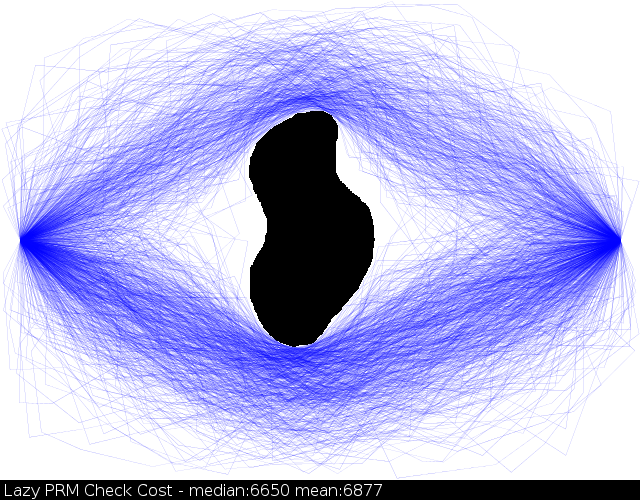
\includegraphics[width=\textwidth]{figs/timegreedy-bean-lambda-00.png}
\caption{Paths with $\lambda = 0$}
\end{subfigure}%
\quad
\begin{subfigure}[b]{0.4\textwidth}
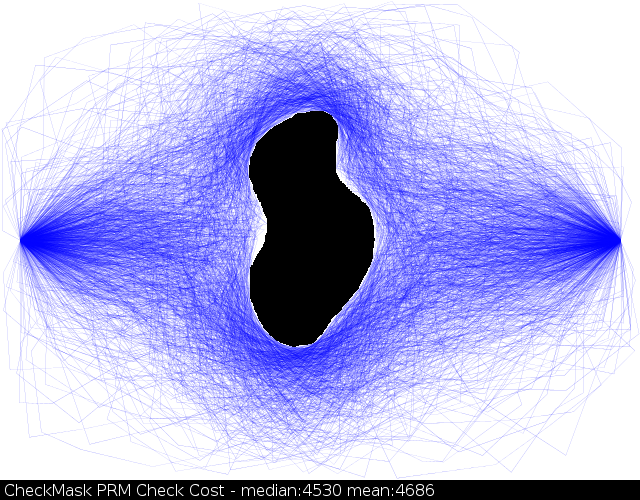
\includegraphics[width=\textwidth]{figs/timegreedy-bean-lambda-10.png}
\caption{Paths with $\lambda = 1$}
\end{subfigure}%
\caption{Examples of paths for a 2d problems
   for different values of $\lambda$.
   As $\lambda$ is increased,
   paths are longer, but are faster to find.}
\label{fig:bean}
\end{figure}

\begin{figure}
\centering
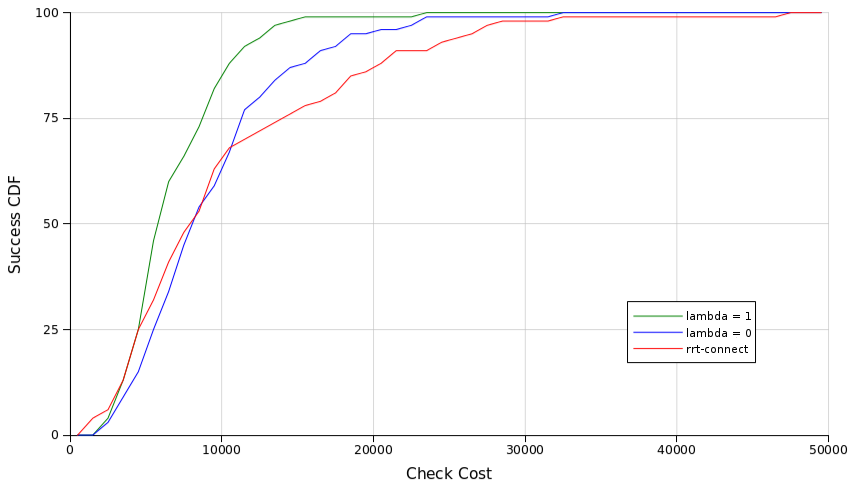
\includegraphics[width=0.8\textwidth]{figs/timegreedy-herbstep1-comparison-cdfs.png}
\caption{Comparison between different algorithms on a HERB problem.
   Must add in ESTs.}
\label{fig:herb-comparison-cdfs}
\end{figure}

\subsection{Future Work}

How to handle the narrow passage problem?
Lots of literature on that, new sampling strategies, etc.
(Toggle PRM, for instance.)



\newpage
\section{The Multi-Space Planning Problem}
\label{sec:multispace}

\begin{itemize}
\item comes from structure of multi-step problem
\item different cfrees
\item but they're very related!
\item inclusions, intersections
\item define multi-space planning problems
\item motivates trajectory reuse
\item examples:
   \begin{itemize}
   \item multi-step manipulation
   \item cached self-checked prms
   \item padded robots (reaching into checkers broad phase stuff)
   \item changing worlds (only check against deltas)
   \item conservative bounding boxes for different grabbed object poses
   \item constantly hypothesizing different sized objects in your hand
   \end{itemize}
\item relation to occupancy grid representations of workspace
   (for deltas, conservative approxs, etc)
\item how is this related to dual-arm stuff?
\item how to fit in CMR?
\end{itemize}

\subsection{Related Work}

Jaillet and Simeon,
\emph{A PRM-based motion planner for dynamically changing environments}
\cite{jaillet2004dynamicprm}.
Explicit dichotomy between static and dynamic parts of the world.
Edges are checked when needed against moving obstacles;
their free-ness with respect to each is cached for the last tested position
for each obstacle.

Gayle, Klingler, and Xavier,
\emph{Lazy Reconfiguration Forest}
\cite{gayle2007lazyreconfigforest}.

Li and Shie,
\emph{An incremental learning approach to motion planning with
      roadmap management}
\cite{li2002incrementalprmmanagement}.
This is the Reconfigurable Random Forest (RRF).
They do ``roadmap management'' to handle changing environments,
and talk about doing some simple bounding-box stuff.

Lien and Lu,
\emph{Planning motion in environments with similar obstacles}
\cite{lien2009similarobstacles}.
This builds a PRM around obstacles in a database,
and then reposes them in a new world.

\subsection{Multiple sub-queries}

\subsection{Shared C-space}

\subsection{Each in a different C-free}

\subsection{Relations between C-frees (inclusion, intersection)}


\newpage
\section{Applying GreedyPRM to MultiSpace: the GreedyMultiPRM}

\begin{itemize}
\item GreedyPRM and multi-space are complementary
\item Apply greeydprm to multi-space problem
\item one planner that learns, can answer arbitrary queries
   in multiple related spaces faster and faster
\end{itemize}


\newpage
\section{A simple task planner using the GreedyMultiPRM}

\begin{itemize}
\item with/without inter-step relations
\item with/without padding
\item with/without self-checked cache
\item with/without relations for changing worlds
\item with/without conservative boxes for grabbed objects
\item constraints:
   \begin{itemize}
   \item handle with separate planner
   \item handle with relaxed constraint, followed by local optimizer
   \end{itemize}
\item run optimizer on paths occasionally and/or before executing
\end{itemize}


\newpage
\section{Conclusion}

meta-graph [future work: probabalistic models]


{\small
\bibliographystyle{abbrv}
\bibliography{pr-refs,siddpubs/siddpubs-conf,siddpubs/siddpubs-journal,siddpubs/siddpubs-misc}
}

\end{document}
